\label{sec:single_crystal_section}

  Добавление в экспериментальную схему (рис. \ref{ris:for_slits}) кристалла - монохроматора
  наглядно демонтирует преимущество использования двумерных спектрально-угловых распределений.
Взаимодействие рентгеновского излучения с кристаллом определяется уже не только
угловой составляющей, но и спектральной.

  Спектрально-угловое распределение после отражения рентгеновского пучка от
  совершенного монокристалла задается выражением:
  \begin{equation} \label{eq:monochromator_spectra}
    P(\vartheta,\lambda) = g_{\lambda}(\lambda)g_{\vartheta}(\vartheta) P(\vartheta - \frac{\lambda - \lambda_1}{\lambda_1}\tg(\theta_B)),
   \end{equation}
где $P$ - соответствует (\ref{eq:KDO_self}), $\lambda_1$ - длина волны излучения, на которую
настраивается экспериментальная схема.

\begin{figure}[H]
  \centering
  \subfloat[]{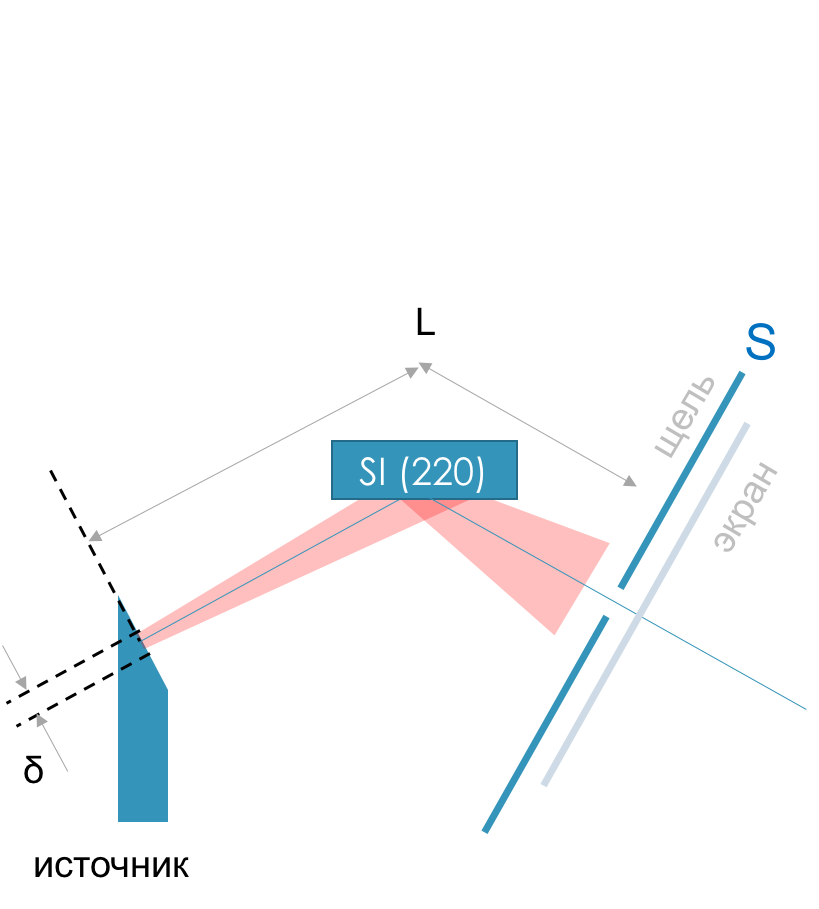
\includegraphics[width=0.45\textwidth]{images/single_crystal_schem.png}\label{ris:single_crystal_schem_lamtet_a}}
  \hfill
  \subfloat[]{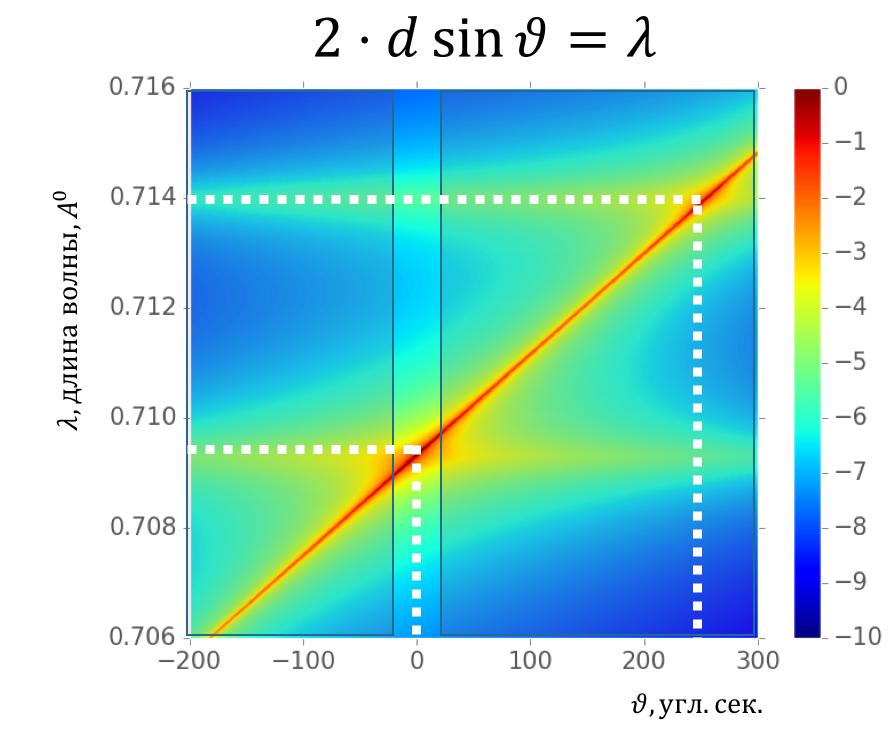
\includegraphics[width=0.45\textwidth]{images/single_crystal_schem_lamtet.png}}

  \caption{Схема однокристального эксперимента (a). Спектрально-угловое распределение
  рентгеновского излучения после отражения расходящегося характеристического излучения
  трубки с $Mo$ анодом от кристалла Si(220). Вертикальная полоса в окрестности
  $\vartheta = 0$ соответсвует угловому диапазону пропускания щелевых коллиматоров.(b)}
  \label{ris:single_crystal_schem_lamtet}
\end{figure}

Рис. \ref{ris:single_crystal_schem_lamtet} наглядно демонстрирует принцип работы
брэгговского монохроматора, когда после взаимодействия с кристаллом, разные
длины волн отражаются под разными углами в соответсвии с законом Вульфа-Брэгга.

Угловая зависимость отраженного монохроматором излучения с учетом прохождения
систем щелей задается следующим образом:

\begin{equation} \label{eq:p_single_crystal}
  P_{single}(\theta) = \sum_{\lambda = -\infty}^{\infty}g_{\lambda}(\lambda) \cdot \sum_{\vartheta = \vartheta_{s1}}^{\vartheta_{s2}}
  g_{\vartheta}(\vartheta) P_M(\vartheta - \frac{\lambda - \lambda_1}{\lambda_1}\tg(\theta_B)),
 \end{equation}
\noindent
где $\vartheta$ - угол падения излучения на кристалл, в случае не расходящегося пучка $\vartheta = 0$, в
случае, например, синхротронного источника $\vartheta \in (-6^o; 6^o) $; $g_{\lambda}(\lambda)$
- спектральная плотность распределения пучка (\ref{eq:source_spectral}); $g_{\vartheta}(\vartheta)$ - угловая плотность
распределения пучка (\ref{eq:source_angle}); $P_M$ - коэффициент отражения от кристалла-монохроматора,
слагаемое $\frac{\lambda - \lambda_1}{\lambda_1}\tg(\theta_B)$ - возникает из
условия Вульфа-Брэгга и описывает свойство разных длинн волн отражатся под разными углами.
 Суммирование проводится, во-первых, в пределах угловой апертуры детектора, которая задается размером
 щелевого коллиматора перед ним, с возможной отстройкой детектора от центрального положения
  $\vartheta_{s1} = \theta - \frac{S}{2L}$, $\vartheta_{s2} = \theta + \frac{S}{2L}$, где
   $S $ - линейный размер щелевого коллиматора, $L$ - расстояние от источника до щели.
 Во-вторых, суммирование осуществляется по всем $\lambda$, из-за свойства детектора не различать разные длины волн.
На рис. \ref{ris:zero_exp} приведен результат измерения углового распределения излучения рентгеновской трубки
после его отражения от неподвижного кристалла кремния Si(220) для разных размеров щелевого коллиматора
в сравнении с результатами моделирования для аналогичных параметров схемы.
Экспериментально измерять такую зависимость можно путем сканирования
детектором со щелью отраженного монохроматором пучка.
